\documentclass{article}
\setlength{\parskip}{\baselineskip}%
\setlength{\parindent}{0pt}%
\usepackage[utf8]{inputenc}
\usepackage{a4wide}
\usepackage{amsmath, amssymb}
\usepackage{enumitem}
\usepackage{qtree}
\usepackage{multicol}
\newcounter{countitems}
\newcounter{nextitemizecount}
\newcommand{\setupcountitems}{%
  \stepcounter{nextitemizecount}%
  \setcounter{countitems}{0}%
  \preto\item{\stepcounter{countitems}}%
}
\makeatletter
\newcommand{\computecountitems}{%
  \edef\@currentlabel{\number\c@countitems}%
  \label{countitems@\number\numexpr\value{nextitemizecount}-1\relax}%
}
\newcommand{\nextitemizecount}{%
  \getrefnumber{countitems@\number\c@nextitemizecount}%
}
\newcommand{\previtemizecount}{%
  \getrefnumber{countitems@\number\numexpr\value{nextitemizecount}-1\relax}%
}
\makeatother    
\newenvironment{AutoMultiColItemize}{%
\ifnumcomp{\nextitemizecount}{>}{3}{\begin{multicols}{2}}{}%
\setupcountitems\begin{itemize}}%
{\end{itemize}%
\unskip\computecountitems\ifnumcomp{\previtemizecount}{>}{3}{\end{multicols}}{}}
\usepackage{graphicx}
\usepackage{listings}
\usepackage{relsize}
\usepackage{amsthm}
\usepackage{dsfont}
\usepackage{wrapfig}
\usepackage{fancyhdr} 
\usepackage{hyperref}
\usepackage[svgnames]{xcolor}
\usepackage[top=70pt,bottom=70pt,left=80pt,right=80pt]{geometry}
\usepackage{subcaption}
\usepackage{verbatim}
\usepackage{wrapfig}
\usepackage{tikz}
\usepackage{float}
\usepackage{csquotes}
\usepackage{sectsty}
\usepackage{apacite}
\usepackage{xcolor}
\newcommand\ddfrac[2]{\frac{\displaystyle #1}{\displaystyle #2}}
\DeclareMathOperator*{\argmin}{arg\,min} 
%\sectionfont{\fontsize{12}{15}\selectfont}
\usepackage{todonotes}
\newcommand{\DL}[1]{\todo[linecolor=blue,backgroundcolor=blue!25,bordercolor=blue,inline]{ \textbf{David}: #1 }}

\lstset{
	breaklines=true,
	columns=fullflexible,
	frame=single,
	numbers=left
}
\pagestyle{fancy}
\fancyhf{}
\cfoot{}
\fancyhead[EL]{\nouppercase\leftmark}
\fancyhead[OR]{\nouppercase\rightmark}
\fancyhead[ER,OL]{\thepage}
\renewcommand{\sectionmark}[1]{\markright{\thesection.\ #1}}
\renewcommand{\subsectionmark}[1]{}

\date{\today}

\begin{document}
\begin{flushright}
Natural Computing \\ 
Assignment 1 \today \\ 
\emph{Stijn de Boer, \textit{s1003731} \\ Ron Hommelsheim \textit{s1000522} \\  David Leeftink, \textit{s4496612} }\\\end{flushright}

% 1
\section{Schemata (0.5 pts)}
\textit{Consider the two schemata A1 = $\#0\#101\#\#\#$, A2 =
$\#\#010\#111$. Which of the two schemata has the highest chance to survive mutation, for a mutation rate $p_m$ = 0.01?} \\ 

The probability that a gene is not mutated is $(1-p_m)$. For a schema to survive, all genes that belong to it should survive. Using $o(S)$ as notation for the order of a schema, this leads to the following formula: $S_m(H)=(1-p_m)^{o(H)}$
This means that schemata with a low order are more likely to survive, as they have less genes that can be mutated.

\begin{table}[H]
    \centering
    \begin{tabular}{|c|c|c|}
        \hline
                 & $A_1$                  &          $A_2$         \\ \hline \hline
        $o(A)$   & $4$                    & $6$                    \\ \hline
        $S_m(A)$ & $(1-0.01)^4 = 0.961$   & $(1-0.01)^6 = 0.941$   \\ \hline
    \end{tabular}
    
\caption{The effect of mutation on two schemata. $o(A)$ is the order of the schema and $S_m(A)$ is the chance of survival under mutation.}
\label{tab:mut}
\end{table}
A1 is more likely to survive therefore.


%2 
\section{Building Block Hypothesis (0.5 pts)}
\textit{Describe a problem where the Building Block Hypothesis does not hold.} \\

The building block hypothesis states that GA's step-wise generate solutions by combining several lower-order schemas (i.e. building blocks). This hypothesis does not hold for every problem: for example, a problem where the reward is 1 for one particular string of genes but 0 for every other gene. An example could be guessing a 4 digit pin-code, where each digits is represented with binary sequences. There is no gradient in the loss function or any other form of information available to guide the GA.

%3 
\section{Selection pressure (1 pts)}
\textit{Given the fitness function $f(x) = x^2$, calculate the probability of selecting the individuals $x = 2, x = 3, and x = 4,$ using roulette wheel selection. Calculate the probability of selecting the same individuals when the fitness function is scaled as follows $f_1 (x) = f (x) + 20$. Which fitness function yields a lower selection pressure? What can you conclude about the effect of fitness scaling on selection pressure?} \\ 

In roulette wheel selection, the probability of an individual being selected is proportional to the ratio of its own fitness and the sum of fitness of the entire population. Put in a formula, it is calculated as $p(s) = \dfrac{f_i}{\sum_i f_i}$. In the problem at hand, we have a population of 3 individuals. Their fitness and probabilities of being selected in roulette wheel selection are: \\
\begin{table}[]
    \centering
    \begin{tabular}{c|c|c|c}
    x    & Fitness  & $p(f)$ & $p(f_1)$\\ \hline \hline
    2    &  4       & 4/29 & 24/89 \\ \hline
    3    &  9       & 9/29 & 29/89\\ \hline
    4    &  16      & 16/29 & 36/89\\    
    \end{tabular}
    \caption{Fitness and probability of selection in roulette wheel selection for the functions $f(x)=x^2$ and $f_1(x)=f(x)+20$}
\end{table}

With $f_1(x)$, the fitness scores are much closer to one another. This causes a lower selection pressure, as a small deviation in value of $x$ causes less difference in the probability of being selected.




%4 
\section{Role of selection in GA's (2 pts)}
The Counting Ones problem amounts to find a bit string whose sum of its entries is maximum. Implement a simple (1 + 1)-GA for solving the Counting Ones problem.
\begin{enumerate}[label=\alph*)]
    \item \textit{Use bit strings of length $l = 100$ and a mutation rate $p = 1/l$. For a run of 1500 iterations, plot the best fitness against the elapsed number of iterations.}
    \begin{figure}[H]
        \centering
        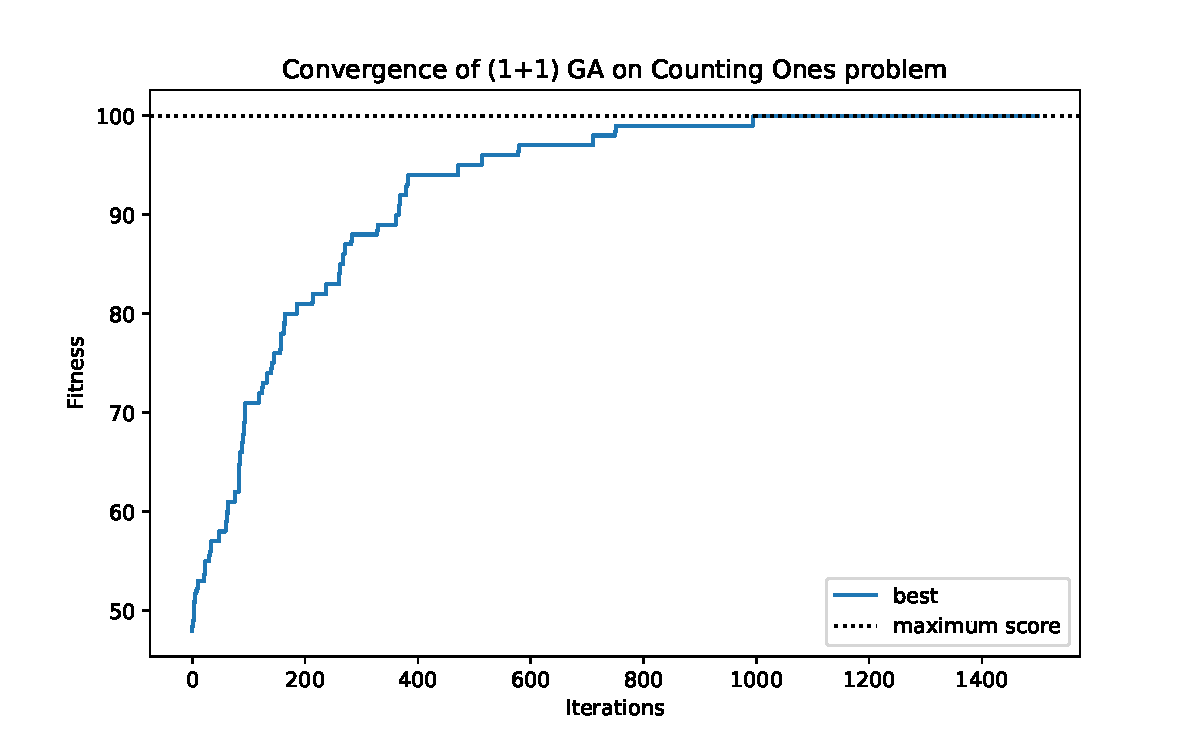
\includegraphics[width=0.9\textwidth]{Assignment 1/Figures/A1_4a.pdf}
        \caption{Convergence of (1+1) GA on Counting Ones problem}
        \label{fig:A1_4a}
    \end{figure}
    \item \textit{Now do 10 runs. How many times the algorithm finds the optimum?}
    The algorithm found the optimum 9/10 runs. With 100 runs, the algorithm found the optimum 92/100 runs. 
    \item \textit{Now replace (c) in the above algorithm with (c'): replace $x$ with $x_m$ . Is there a difference in performance when using this modification? Justify your answer} \\ 
    
    With the alteration, the GA performs a lot worse. The fitness of the determined solution fluctuates around the initial fitness. 0/10 runs have converged to the optimum. Repeating the experiment with 100 runs shows that 0/100 runs have converged. We can conclude that rule c is an important addition in the (1+1) GA algorithm, as the algorithm forgets the best solution found thus far otherwise.
    \begin{figure}[H]
        \centering
        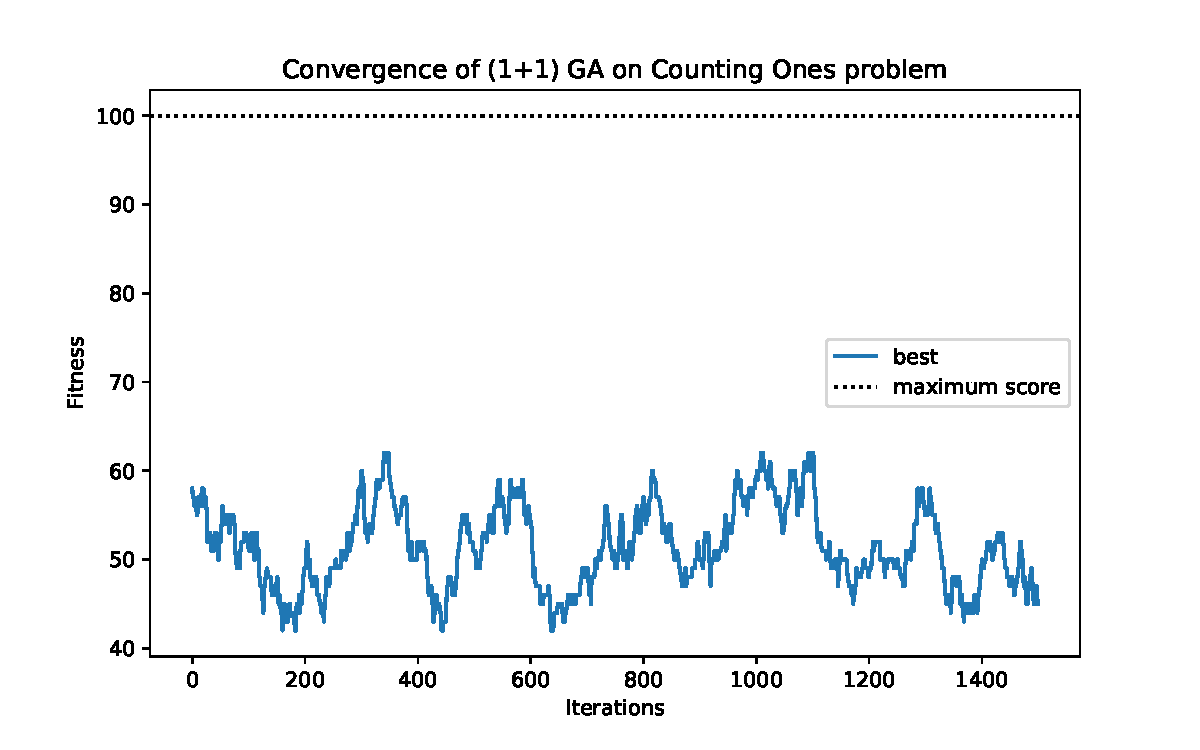
\includegraphics[width=0.9\textwidth]{Assignment 1/Figures/A1_4c.pdf}
        \caption{Convergence of (1+1) altered GA on Counting Ones problem}
        \label{fig:A1_4c}
    \end{figure}
\end{enumerate}

%5 
\section{Evolutionary strategies vs local search (1 pts)}
\textit{Consider a (1+5) ES. How does this differ from the (1+1) ES in how the search space is explored when optimizing a function? How does the (1+$\lambda$) ES strategy behave with respect to the value of $\lambda$ when compared to greedy algorithms? } \\ 

A (1+5) ES algorithm represents a population where 1 member (the best) is chosen to survive to the next generation, in which 5 new children are initialized. The (1+5) ES is different from a (1+1) ES, because in a (1+1) ES at each iteration the best solution is kept and one child is added to the population. This means that if the child outperforms the parent, it replaces the parent. If the child does not outperform the parent, it is replaced by another child. As there is one child, at each time one direction of search in the real-valued vector space is explored.

Compared to a (1+5) ES there is a large difference, since there are now 5 children that can potentially replace the parent. At each iteration, the best of the 5 children and parent is chosen to be the new parent. With 5 children at each iteration, 5 directions of search in the real-valued vector space are explored.

Since ES are concerned with optimizing real valued vectors (such as weights), we can compare the optimization behaviour with standard hill-climbing methods such as greedy or gradient-descent. Whereas these methods \textit{always} take a step in the new direction, as (1+$\lambda$) ES only takes this step if the fitness of the step is actually improved. The higher the value of $\lambda$, the more informed the next step of the iteration becomes as more directions in the search space are explored. This can be advantageous, as this allows the algorithm to 'remember' certain solutions: it does not accidentally forget the best solution due to an unfortunate sequence of mutation, recombination and cross-over operations. However it can also cause the system to be more likely to be trapped in local optima/minima. 

The procedure will pick the best of the $\lambda$ children at the next time step, because of the '1' in (1+$\lambda$). As we let $\lambda$ go to infinity, all \textit{possible} children will be evaluated, and of those children the best is picked. This means that the (1+$\lambda$)-ES algorithm becomes a greedy algorithm if we let $\lambda \to \infty$, because greedy algorithms perform a sequence of locally optimal steps. 


%6 
\section{Memetic algorithms vs simple EAs (2.5 pts)}
The implementation of the standard EA and of the memetic algorithms are made using the python library DEAP \cite{deap}. The implementation can be found at \url{https://github.com/DavidLeeftink/NaturalComputing2021/blob/main/Assignment\%201/A1\%20Natural\%20Computing.ipynb}. Jupyter notebooks can be run by downloading the conda package; further instructions on how to install the notebook are detailed at \url{https://jupyter.org/install}. All other required packages are automatically installed by executing the code. The required data of the cities is given in the GitHub is as well, and can be downloaded to run the program. 

\begin{enumerate}[label=\alph*)]
    \item \textit{Implement a variant of this algorithm based on memetic algorithms.} \\
    
    \begin{figure}[H]
        \centering
        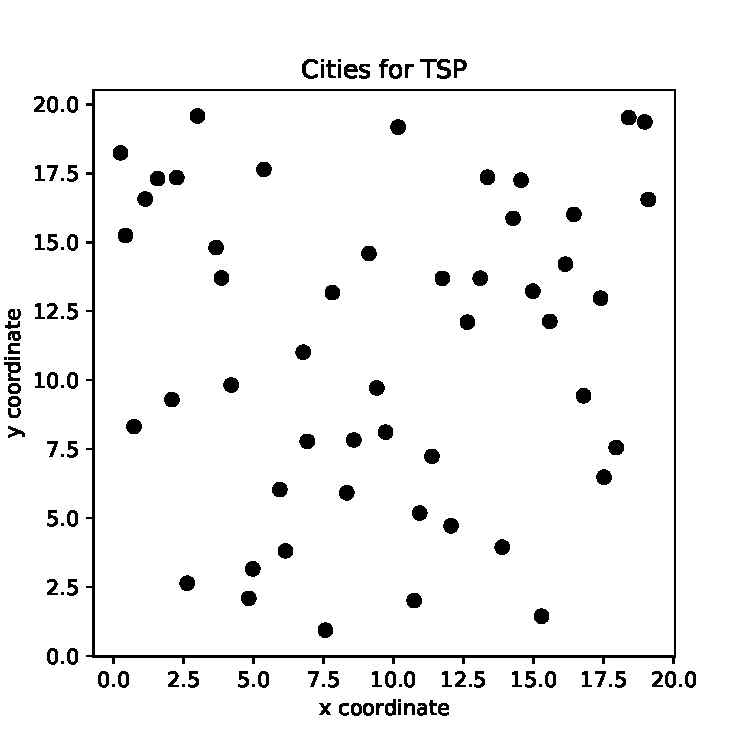
\includegraphics[width=0.5\textwidth]{Assignment 1/Figures/A1_6a.pdf}
        \caption{Given cities to be connected for the TSP problem.}
        \label{fig:A1_6a}
    \end{figure}

    \item \textit{On the TSP problem are memetic algorithms more effective than the simple EA’ s? } \\
    As shown in figure \ref{fig:A1_6b1} and \ref{fig:A1_6b2}, the memetic algorithm converges faster to a lower distance (higher fitness). The memetic algorithm was chosen to run for only 100 iterations, as it converges quickly and requires a much higher computation per iteration. After 100 iterations, it has reached a minimum distance near 150: we believe this might be the global optimum as well. The simple EA performs a lot worse: after 1500 iterations, the best distance is near 250. 
    
    \begin{figure}[H]
        \centering
        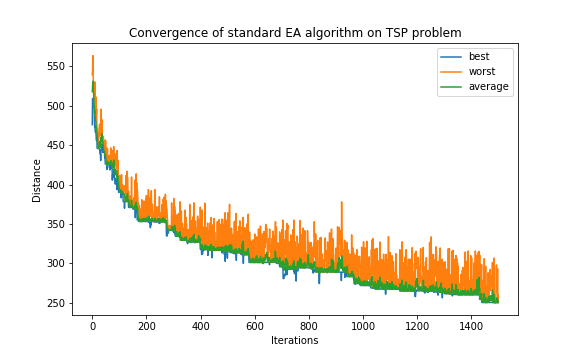
\includegraphics[width=0.7\textwidth]{Assignment 1/Figures/A1_6b1.png}
        \caption{Convergence of standard EA algorithm on the given data in the exercise.}
        \label{fig:A1_6b1}
    \end{figure}  
    \begin{figure}[H]
        \centering
        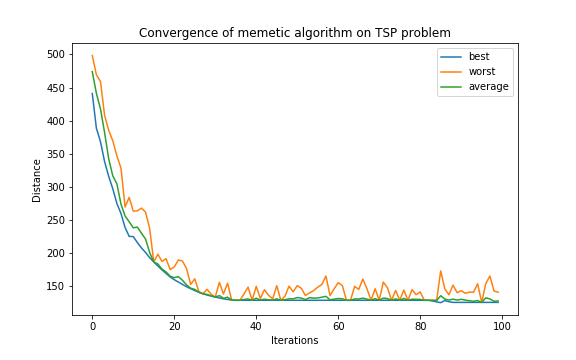
\includegraphics[width=0.7\textwidth]{Assignment 1/Figures/A1_6b2.png}
        \caption{Convergence of memetic algorithm on the given data in the exercise.}
        \label{fig:A1_6b2}
    \end{figure}
    
    For the second data set, we have chosen the data set \texttt{27\_cities}\footnote{elib.zib.de/pub/mp-testdata/tsp/tsplib/tsp/bays29.tsp}, which contains (unlike the name suggests) 29 cities in Germany (Bavaria). The results of both algorithms are similar to the results found on the first data set. They are found in figure \ref{fig:A6_6c1} and \ref{fig:A6_6c2}.
   
    
    \begin{figure}[H]
        \centering
        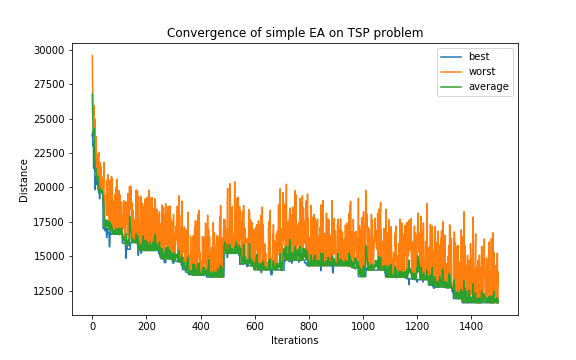
\includegraphics[width=0.7\textwidth]{Assignment 1/Figures/A1_6c1.png}
        \caption{Convergence of standard EA algorithm on the Bavarian Cities in Germany. }
        \label{fig:A1_6c1}
    \end{figure}  
    \begin{figure}[H]
        \centering
        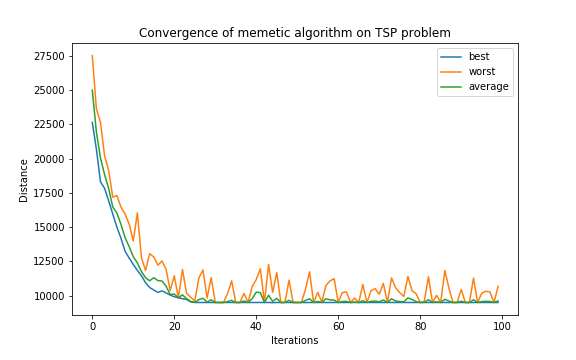
\includegraphics[width=0.7\textwidth]{Assignment 1/Figures/A1_6c2.png}
        \caption{Convergence of memetic algorithm on the Bavarian Cities in Germany. }
        \label{fig:A1_6c2}
    \end{figure}
    
    The results are sensible, as the memetic algorithm is performing its search in a reduced search space namely only the local optimal solutions.  Comparing these findings with existing literature, we find that the memetic algorithm is not preferred in every TSP problem, however. An important factor is the size of the problem  \cite{merz2001memetic}. In addition, \cite{merz2001memetic} claim that memetic algorithms are good at exploiting the correlation structure of landscapes. If fitness landscapes are smooth, i.e. a small change of ordering in cities leads to a small change in fitness, memetic are the preferred choice.
    \citeA{contreras2015automatic} show that standard EA algorithms are competitive in terms of performance for problems where $N$ is high. 
\end{enumerate}

%7 
\section{Genetic programming representation (0.5 pts)}
\textit{Give a suitable function, terminal
set and s-expression for the following logical and mathematical formulas}.
\begin{enumerate}[label=\alph*)]
    \item $(y \land true) \to ((x \lor y) \lor (z \leftrightarrow (x \land y)))$ \\
    Function set: $\{\neg, \land, \lor, \to,\leftrightarrow \}$ \\
    Terminal set: $\{x,y,z,true, false\}$ \\
    LISP S-expression: $(\to \:(\land \: y \: true) (\lor \:(\lor \: x \: y) \: (\leftrightarrow \: z \: (\land \: x \: y)) ) )$ \\
    Tree representation: 
    \Tree[.\to . [.\land . [.y ]
              [.true ]]
          [.\lor . [.\lor . x y  ]
                [.\leftrightarrow. [z. [.\land . x y  ]] ]]]
    \item $0.234 \cdot z + x–0.789$ \\ 
    Function set: $\{+, *, -, \div\}$ \\ 
    Terminal set: $\{x, z\} \cup \mathbb{R}$ \\ 
    LISP s-expression: $(+ \:(*\:0.234 \:z) \:(- \: x \:0.789)  )$ \\
    Tree representation: 
    \Tree[.+  [.* [.0.234 ]
              [.z ]]
          [.-  [.x ]
                [.0.789. ]]]
\end{enumerate}

%8
\section{Genetic programming behaviour (2 pts)}
\textit{Implement a GP program for finding a
symbolic expression } \\ 

The implementation of the program is made using the python library DEAP \cite{deap}. The implementation can be found at \url{https://github.com/DavidLeeftink/NaturalComputing2021/blob/main/Assignment\%201/deap_experiment.ipynb}. Jupyter notebooks can be run by downloading the conda package; further instructions on how to install the notebook are detailed at \url{https://jupyter.org/install}. All other required packages are automatically installed by executing the code. Note that parts of code are copied from the DEAP package, to prevent additional imports. We do not claim to have written any of the functionality by the package, and merely use it to compute the optimal genetic programming solution to the given data.

The algorithm is run with the following parameters: a population size of 1000, 50 generations, $p_m = 0$, $p_c = 0.7$. In addition, we have used tournament selection with $K=3$. 

The results are shown in figure \ref{fig:A1_8a1} and \ref{fig:A1_8a2} for the best generation sizes vs. generation and maximum fitness vs. generations respectively. The best solution found by the program is the following expressions: \texttt{mul(add(mul(mul(x, x), x), x), sub(x, -1))}. This corresponds to the function $f(x) = x^4+x^3+x^2+x$. To validate the solution, the function is visually displayed together with the observations in figure \ref{fig:A1_8a3}. This shows that the solution fits through the observations very well, and no difference between the solution and observation can be seen by eye. The good performance is validated by the small mean absolute error. Note that the optimal solution is already found at generation 6. 

Whereas the mean absolute error is converging to 0, the max size of the solutions as a function of generations is increasing. This means that the longer the algorithm is run, the more complex the solutions become, and is known as the 'bloat' phenomenon (also referred to as survival of the fattest). This is likely to cause the system to overfit on the observations, due to a lack of parsimony of the model. In the end, we are interested in the simplest model that can explain the same data as well as any more complex model. In real-life applications, it would therefore be preferred to use cross-validation or use complexity penalties in model selection, to ensure that the model is able to generalize well to other values of $x$ that are not seen in the observed data. 

\begin{figure}[H]
    \centering
    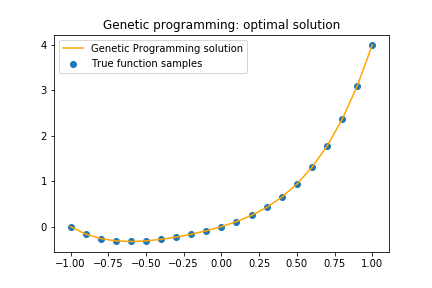
\includegraphics[width=0.7\textwidth]{Assignment 1/Figures/A1_8a3.png}
    \caption{Genetic programming: visualization of the solution found. The final function found by the program: \texttt{mul(add(mul(mul(x, x), x), x), sub(x, -1))}. This corresponds to: $f(x) = x^4+x^3+x^2+x$.}
    \label{fig:A1_8a3}
\end{figure}

 \begin{figure}[H]
    \centering
    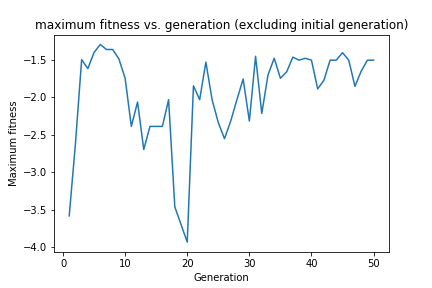
\includegraphics[width=0.7\textwidth]{Assignment 1/Figures/A1_8a2.png}
    \caption{Maximum fitness as a function of generations (the initial generation is excluded for clearness of the plot)}
    \label{fig:A1_8a2}
\end{figure}

 \begin{figure}[H]
    \centering
    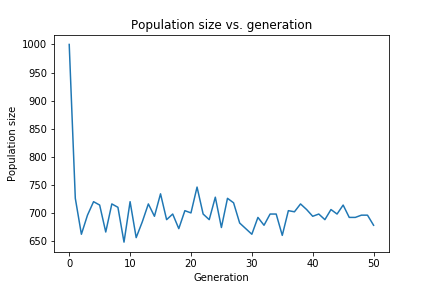
\includegraphics[width=0.7\textwidth]{Assignment 1/Figures/A1_8a1.png}
    \caption{Best of generation size as function of generations for the Genetic Programming algorithm.}
    \label{fig:A1_8a1}
\end{figure}
    

 
 
 
\bibliographystyle{apacite}
\bibliography{references.bib}

\end{document}